%!TEX encoding = UTF-8 Unicode
%!TEX root = ../lect-w13.tex
%%%

% \ifkompendium\else
% \begin{Slide}{Denna läsvecka nr 13}
%     \begin{itemize}
%         \item Föreläsningar: Tentatips, repetition.
%         \item Resurstider: Projektarbete, uppsamling.
%         \item Labbtider: Projektredovisning.
%     \end{itemize}
% \end{Slide}


% \begin{Slide}{Nästa läsvecka nr 14: sista ordinarie veckan innan jul}
%     \begin{itemize}
%         \item Föreläsningar: 
%         \begin{itemize}
%             \item På begäran: grumligt + nyfiken. 
%             \item Repetition.
%             \item Utblick: Scala 3, kommande kurser.
%         \end{itemize}
%         \item Resurstider: \Alert{Uppsamling!}
%         \item Ingen labb på schemat.
%     \end{itemize}
% \end{Slide}

% \begin{Slide}{Nästa läsvecka nr 14: sista ordinarie veckan innan jul}

%   \begin{itemize}
%     \item Du \Alert{måste} ha alla obl. moment klara för att få påbörja fördjupningskursen.
%     \item Fördjupningskursen är förkunskaper till många kurser.
%     \item Du \Alert{måste} ha alla obl. moment klara för att få tentera. 
%     \item \Alert{Uppsamling} på \Emph{resurstider} för att redovisa rest-moment. \\ VIKTIGT: gör klart och redovisa \Alert{alla} labbar + projektet

%     \item Erfarenhet visar att det är på \Emph{första} \Alert{ordinarie} tentan du har din bästa chans! Gör ditt bästa den 13/1 kl 8-13 i MA:9!
    

%     \item Undantag: Du behöver inte klara tentan för att få påbörja fördjupningskursen \Alert{direkt efter jul} (men om du måste vänta till nästa år pga restlabb måste du först klara tentan)


%     \item Föreläsningarna fortsätter med repetition, ''grumligt'', ämnen på begäran, utblick, m.m.
%     \item Dubbelkolla snapshot dina registreringar: cs.lth.se/pgk/sam
%   \end{itemize}

% \end{Slide}

% \Subsection{Grumligt + Nyfiken}
% \begin{Slide}{Grumligt + Nyfiken}
%     \begin{itemize}
%         \item \Alert{Grumligt}-lådan: om du tycker något viktigt begrepp i kursen är svårt så skriv en lapp och lägg i denna låda.
%         \item \Emph{Nyfiken-på}-lådan: om du vill veta mer om något begrepp som är relaterat till kursen så skriv en lapp och lägg i denna låda.
%     \end{itemize}
%     OBS! Endast ETT begrepp per lapp.
% \end{Slide}


% \Subsection{Gruppbonus från kontrollskrivning 2019}

% \begin{Slide}{Gruppbonus från kontrollskrivning 2019} 
%     \SlideFontSize{6.5}{8.2}
% \begin{tabular}{l c l}
%     Grupp & bonus & poäng \\\hline
% D1.01a: & 3 & 1,2,2,3,4,4  \\
% D1.01b: & 3 & 0,1,3,3,4,5  \\
% D1.02a: & 3 & 1,2,2,3,4,5  \\
% D1.02b: & 2 & 0,2,2,4      \\
% D1.03a: & 2 & 1,1,2,3,4    \\
% D1.03b: & 2 & 1,1,2,2,3    \\
% D1.04a: & 2 & 1,2,2,3,4    \\
% D1.04b: & 3 & 2,2,3,3,4    \\
% D1.05a: & 3 & 2,2,2,3,5    \\
% D1.05b: & 3 & 1,2,2,3,5    \\
% D1.06a: & 3 & 1,1,3,4,5    \\
% D1.06b: & 3 & 1,2,2,5,5    \\
% D1.07a: & 2 & 1,1,2,3,4    \\
% D1.07b: & 2 & 2,2,2,3,3    \\
% D1.08a: & 2 & 2,2,2,2,2    \\
% D1.08b: & 3 & 3,3,3,4,4    \\
% D1.09a: & 3 & 1,2,3,5      \\
% D1.09b: & 2 & 0,2,2,3,4    \\
% D1.10a: & 2 & 1,1,2,4,4    \\
% D1.10b: & 2 & 1,1,3,3,4    \\
% D1.11a: & 2 & 1,1,1,2,3,4  \\
% D1.11b: & 2 & 1,2,2,2,3    \\
% D1.12a: & 3 & 2,2,3,3,3,4,4\\
% D1.12b: & 2 & 1,1,2,3,5    \\
% \end{tabular}
% \end{Slide} 
% \fi


\Subsection{Repetition på begäran}

\newcommand{\Vecka}[1]{\hfill\href{https://fileadmin.cs.lth.se/pgk/lect-w#1.pdf}{w#1}}

% \begin{Slide}{Repetitionsämnen 2020}
% Gör en lista på saker du behöver repetera.\\Exempel på önskade repetitionsämnen från tidigare år:
% \begin{itemize}\SlideFontSmall
%   \item closure (''fångad variabelrymd'') \Vecka{03}
%   \item Skillnad på objekt och singelobjekt? \Vecka{04}
%   \item Mönstermatchning. \Vecka{06}
%   \item \code{Option}  \Vecka{06}
%   \item \code{Try} med stort T  \Vecka{06}
%   \item \code{enum}: när och hur? eller case-klass? \Vecka{07}
%   \item När använda vilken sekvenstyp? \Vecka{07}
%   \item Typhärledning. \Vecka{08}
%   \item komposition eller arv?  \Vecka{10}
% \end{itemize}  
% \end{Slide}

\begin{Slide}{Repetitionsämnen på begäran 2022}
\begin{enumerate}\SlideFontSmall
   \item namnanrop, värdeanrop \Vecka{03}
   \item funktionsvärde, funktionstyp och thunk \Vecka{03}
   \item \code{--classpath} \Vecka{04}
   \item \code{import} \Vecka{04}
   \item \code{Option} \Vecka{06}
   \item \code{Try} \Vecka{06}
   \item \code{enum} \Vecka{07}
   \item avlusning, läsa felmeddelande \Vecka{08}
   \item \code{given using} \Vecka{11}
\end{enumerate}  
\end{Slide}

\begin{Slide}{Några extra önskemål från tidigare år (i mån av tid)}
\begin{enumerate}\SlideFontSmall
  \item Closure (''fångad variabelrymd'') \Vecka{03}
  \item Skillnad på objekt och singelobjekt? \Vecka{04}
  \item Mönstermatchning. \Vecka{06}
  \item När använda vilken sekvenstyp? \Vecka{07}
  \item Typhärledning. \Vecka{08}
  \item Komposition eller arv?  \Vecka{10}
\end{enumerate}  
\end{Slide}


\begin{Slide}{Några tumregler/tips vid val av abstraktion}\SlideFontSmall
Om du skulle behöva samla både attribut och metoder:
Extensionsmetod, singelobjekt, case-klass, klass, trait eller abstrakt klass, eller enum?
\begin{itemize}\SlideFontTiny
\item Om du vill lägga till en metod på befintlig typ utan att ha nya attribut, använd \code{extension}.
\item Använd \code{object} om du behöver samla metoder (och variabler) i en modul som bara finns i en upplaga. Du får lokal namnrymd och punktnotation på köpet.
\item Behöver du modellera \Emph{oföränderlig data}, använd en \code{case class} eller \code{enum}.  
\item Om du vill ha uppräknade värden som du vill kunna iterera över och matcha på i förseglad struktur, med värden i egen namnrymd, använd \code{enum}.
\item Med \code{case class} och \code{enum} Du får då även innehållslikhet och en massa annat godis på köpet!
\item Behöver du \Alert{förändringsbart tillstånd} \Eng{mutable state} använd en vanlig \code{class}. Det normala är att det föränderliga tillståndet (de attribut som är föränderliga) är \code{private} eller \code{protected} och att all uppdatering och avläsning av tillståndet sker indirekt genom metoder (getters/setters/...).
\item Behöver du en abstrakt bastyp använd en \code{trait}, speciellt om du vill ha möjlighet till inmixning.  Om du vill förhindra inmixning eller underlätta användning från Java, använd \code{abstract class}. 
\end{itemize}
\end{Slide}


% \begin{Slide}{Tips om hur man läser en specifikation}\SlideFontSmall
% När du läser en specifikation av en klass, en trait, eller ett singelobjekt:
% \begin{itemize}
% \item Tänk igenom vilket ansvar olika delar av koden har
% \item Vad håller klassen reda på? \\$\rightarrow$ Ledtrådar till attribut
% \item Vad ska klassen göra/räkna ut? \\$\rightarrow$ Ledtrådar till metoder och deras algoritm
% \item Vilka andra klasser har nytta av denna metod? \\$\rightarrow$ Ledtrådar till hur klasserna samverkar för att lösa uppgiften
% \end{itemize}
% Rita gärna en bild med ett specifikt exempel på vilken data som olika instanser håller reda på och fundera på hur data skapas/beräknas/förändras
% \end{Slide}


\begin{Slide}{Tips om val av samling}\SlideFontSmall

Det är ofta enklare med oföränderliga samlingar med oföränderliga element och skapa nya samlingar vid förändring. Men för vissa algoritmer blir det enklare eller effektivare om du ändrar på plats i förändringsbar samling.

\begin{itemize}
\item Behöver du hantera värden i sekvens?
\begin{itemize}\SlideFontTiny
\item Om du klarar dig utan förändring av innehållet efter konstruktion:\\
\code{val}-referens till \code{Vector}
\item Om du behöver ändra innehåll men \Alert{inte} antal element:\\
\code{val}-referens till \code{Array}
\item Om du behöver ändra innehåll \Alert{och} antal element:
\\ \code{var}-referens till \code{Vector} och t.ex. metoden \code{patch}, eller \\
\code{val}-referens till \code{ArrayBuffer} och t.ex. metoden \code{insert}
\end{itemize}

\item Behöver du hantera värden \code{x} som ska vara unika?
\begin{itemize}\SlideFontTiny
\item Oföränderlig: \code{  Set}
\item Förändringsbar: \code{val}-referens till \code{scala.collection.mutable.Set}
\end{itemize}

\item Behöver du leta upp värden \code{x:Int} utifrån en nyckel av t.ex. String?
\begin{itemize}\SlideFontTiny
\item Oföränderlig: \code{Map[String, Int] }
\item Förändringsbar: \code{val}-referens till \code{scala.collection.mutable.Map[String, Int]}
\end{itemize}


\end{itemize}
\end{Slide}

% \begin{Slide}{ArrayBuffer}
% Ändra på plats: update, insert, remove, append
% {\SlideFontTiny

% \vspace{2.5em}\begin{tabular}{@{}p{4.2cm}  p{6.5cm}}
% \texttt{xs(i) = x \newline xs.update(i, x)} & Replace element at index i with x. \newline Return type Unit.\\   \cline{1-2}

% \texttt{xs.insert(i, x)\newline xs.remove(i)} & Insert x at index \texttt{i}. Remove element at i. \newline Return type Unit.\\   \cline{1-2}

% \texttt{xs.append(x)~~~xs~+=~x} & Insert x at end.  Return type Unit.\\   \cline{1-2}

% \texttt{xs.prepend(x)~~x~+=:~xs} & Insert x in front.  Return type Unit.\\   \cline{1-2}

% \texttt{xs -= x} & Remove first occurance of x (if exists). \newline Returns xs itself. \\\cline{1-2}

% \texttt{xs ++= ys} & Appends all elements in ys to xs and returns xs itself. \\

% \end{tabular}
% }

% \end{Slide}


\Subsection{Tentatips}

\begin{Slide}{Före tentan:}\SlideFontSmall
\begin{enumerate}
\item Repetera övningar och labbar i kompendiet.
\item Läs igenom föreläsningsanteckningar.
\item Studera \Emph{snabbref} \Alert{mycket noga} så att du vet vad som är givet och var det står, så att du kan hitta det du behöver snabbt.
\item Skapa och \Emph{memorera} en personlig \Emph{checklista} med programmeringsfel du brukar göra, som även inkluderar småfel, så som glömda parenteser och semikolon, och annat som en kompilator/IDE normalt hittar.
\item Tänk igenom hur du ska disponera dina 5 timmar på tentan.
\item Gör minst en extenta som om det vore \Alert{skarpt läge}:
\begin{enumerate}\SlideFontTiny
\item Avsätt 5 ostörda timmar (stäng av telefon, dator etc).
\item Inga hjälpmedel. Bara snabbref.
\item Förbered dryck och tilltugg.
\end{enumerate}
\end{enumerate}
\end{Slide}

\begin{Slide}{På tentan:} \SlideFontTiny
\begin{enumerate}
\item Läs igenom \Alert{hela} tentan först. \\ \Emph{Varför?} Förstå helheten. Delarna hänger ihop.
\item Notera och begrunda specifika begrepp och definitioner. \\ \Emph{Varför?} Begreppen är avgörande för förståelsen av uppgiften.
\item Notera förenklingar, antaganden och specialfall. \\ \Emph{Varför?} Uppgiften blir mkt enklare om du inte behöver hantera dessa.
\item \Alert{Fråga} tentamensansvarig om du inte förstår uppgiften -- speciellt om det finns misstänkta felaktigheter eller förmodat oavsiktliga oklarheter. \\ \Emph{Varför?} Det är inte lätt att konstruera en ''perfekt'' tenta. \\ Du får fråga vad du vill, men det är inte säkert du får svar :)
\item Läs specifikationskommentarerna och metodsignaturerna i alla givna klass-specifikationer \Alert{mycket noga}. \\ \Emph{Varför?} Det är ett vanligt misstag att förbise de ledtrådar som ges där.
\item Återskapa din memorerade personliga checklista för vanliga fel som du brukar göra och avsätt tid till att gå igenom den på tentan. Varje fix plockar poäng!
\item Lämna in ett försök även om du vet att lösningen inte är fullständig. Det gäller att plocka så många poäng det går. En ofullständig lösning kan ändå ge poäng.

\item Om du har svårigheter kan det bli kamp mot klockan. Försök hålla huvudet kallt och prioritera utifrån var du kan plocka flest poäng. Ge inte upp! Ta en kort äta-dricka-paus för att få mer energi!

\end{enumerate}
\end{Slide}

\ifkompendium\else

\begin{Slide}{Planeringstips}\SlideFontTiny
Exempel på saker som du kan lägga in tid för i din julpluggkalender:
\begin{enumerate}
\item Ta reda på vad just \Alert{du} behöver träna på!
\item Välja ut övningar att repetera.
\item Repetera övning X, Y, Z, ... Både läsa och skriva kod. Fundera på typ och värde.
\item Välja ut labbar att repetera.
\item Repetera labb X, Y, Z, ... Lär dig ''trick'' och ''mönster''.
\item Träna på att skriva program med papper och penna.
\item Gör så många extentor du orkar, simulera ''skarp läge''.
\item Gör en checklista med vanliga fel och misstag som du brukar göra.
%\item Det finns inte så många Scala-extentor, men du kan också göra Java-extentor och lösa vissa delar i Scala och vissa delar i Java beroende på vad du behöver träna på.

\item Läsa igenom de extentor i Scala och Java som du väljer att inte göra ''i fiktivt skarpt läge'' och studera generella mönster och typiska trick.
\end{enumerate}
\end{Slide}

\begin{Slide}{Tentans struktur}
\begin{itemize}\SlideFontSmall
\item Del A 20\%:\\\Emph{Evaluera uttryck} där du ska \Alert{ange typ och värde}
\begin{itemize}\SlideFontTiny
\item Testar förståelse av variabler, uttryck, samlingar, algoritmer, arv, etc.
\item Det är bra/nödvändigt att skriva ner delsteg och variablers värden, då det kan vara svårt att tänka ut svaren direkt i huvudet.
\item Ev. ''rättningströskel'': \textit{Om du på del A erhåller färre poäng än vad som krävs för att nå upp till en bestämd ''rättningströskel'', kan din tentamen komma att underkännas utan att del B bedöms.}
\end{itemize}


\item Del B 80\%:\\\Emph{Skriva kod} som uppfyller \Alert{krav och design}
\begin{itemize}\SlideFontTiny
\item Testar att du själv kan skapa kod med delar som samverkar
\item Testar förmåga att gå från indata-utdata till algoritm \\
 givet: ledtrådar, design, ev. skiss på lösning, ev. pseudokod etc.
\item En av uppgifterna ska besvaras i Java, men den testar mer än bara Java-kompetens. Det är bättre att svara i Scala-liknande Java om du är osäker på Java än att inte lämna in alls.
\end{itemize}
\item Blanka inlämningar ger 0 poäng; det är alltid bättre att försöka än att lämna in blankt. Lämna inte in kladdpapper eller dubbla lösningar.
\end{itemize}
\end{Slide}


\begin{Slide}{Vad kommer på tentan?}
\begin{itemize}
\item Grundläggande begrepp och det som tränas på grundövningar och labbar är basen för att bli godkänd.
\item Begrepp, föreläsningsbilder och övningar som är markerade \Emph{''fördjupning''} krävs ej för att klara tentan men ökar förståelsen och hjälper dig att nå högre betyg.
\item Det är helt ok på tentan om du väljer en \Emph{enkel lösning med basala begrepp} \Alert{som fungerar bra}, i stället för en kortare/elegantare/mer avancerad lösning.
\item Extra-övningarna i läsvecka 14 ingår ej på tentan.
\end{itemize}
\end{Slide}



% \begin{Slide}{Vad kommer på tentan? (Bild 2 av 4)}\SlideFontTiny
% \hspace{-1em}\begin{minipage}{1.0\textwidth}
% \vspace{1em}\begin{tabular}{l | l | l}
% \textbf{Modul} & \textit{Ingår t.ex.}& \textit{Avgränsning} (ej krav)\\\hline
% \hline
% Introduktion & sekv., alt., rep., abstraktion, & De Morgans lagar \\
%              & uttryck, aritmetik, slumptal, &    stränginterpolatorerna s, f\\
%              & strängar, grundtyper, Unit, ()  & Float, Byte, Short \\
%              & skillnad mellan heltal och flyttal \\
%              & variabler, for, while, if & \\ %hex-literaler, backticks\\
% \hline
% Program      & main, args, utdata, println, indata & io.StdIn.readLine\\
%              & Vector, Array, indexering,  &     \\
%              & iterera över samling, for-uttryck, yield, \\
%              & Range, map, foreach, sats vs uttryck & \\
%              & SWAP, SUM, MIN-MAX, MIN-INDEX & \\
% \hline
% Funktioner    & definiera, anropa, parameter, argument  & skapa kontrollstruktur \\
%               & returtyp, namngivna arg., defaultarg  & namnanrop\\
%               & apply,  scala.util.Random & slumptalsfrö\\
%               & anonyma funktioner (lambda)  & stegad funktion, rekursion\\
%               & map/foreach med anonym funktion & \\

% \end{tabular}
% \end{minipage}
% \end{Slide}


% \begin{Slide}{Vad kommer på tentan? (Nild 3 av 4)}\SlideFontTiny
% \hspace{-2em}\begin{minipage}{1.0\textwidth}
% \begin{tabular}{l | l | l}
% \textbf{Modul} & \textit{Ingår t.ex.}& \textit{Avgränsning} (ej krav)\\\hline
% Objekt      & singelobjekt, attribut, medlem, metod, & isInstanceOf (anv. match istället) \\
%             & tillstånd, synlighet, skuggning, block, & scaladoc, javadoc, jar \\
%             & punktnotation, namnrymd,  & paket, import, PixelWindow \\
%             & lazy val, io.Source.fromFile  &  \\
%             & tupler, multipla returvärden &  \\
% \hline

% Klasser     &  klass, case-klass, instans, new, konstruktor, & null, alternativ kontruktor, \\
%             &  this, inkapsling, accessregler, kompanjon, & private[this] \\
%             &  klassparameter, fabriksmetod, getter, setter, & \\
%             &  referenslikhet och innehållslikhet,    & \\
%             &  förändringsbara och oföränderliga instanser & \\
% \hline

% Sekvenser  &  skapa ny samling, samlingsmetoder, &   List (ofta bra med Vector istället), \\
%             & skapa ny variant av oföränderlig samling, & tids- och minneskomplexitet, \\
%             &  heltalsregistrering i Array, linjärsökning, & Scanner, StringBuilder,\\
%             &  förändringsbar sekvens, ArrayBuffer & deklarera repeterade parametrar\\
% \hline

% Mängder, & förändrinsbar och oföränderlig mängd,  & spara/läsa till/från fil \\%serialisering, \\
% tabeller & förändrinsbar och oföränderlig tabell, & \\%java.nio.file\\
%          & registrering av godtyckliga värden i tabell  & \\
% \hline

% \end{tabular}
% \end{minipage}
% \end{Slide}


% \begin{Slide}{Vad kommer på tentan? (Bild 4 av 4)}\SlideFontTiny
% \hspace{-2em}\begin{minipage}{1.0\textwidth}
% \begin{tabular}{l | l | l}
% \textbf{Modul} & \textit{Ingår t.ex.}& \textit{Avgränsning} (ej krav)\\\hline

% Matriser,     & indexering i nästlade strukturer & \\
% typparametrar & nästlad for-sats, matriser i Java  & \\
%               & använda generiska strukturer & skapa generiska strukturer\\
% \hline

% Arv         &  bastyp, subtyp, trait, abstrakt,   & inmixning, \\
%             &  Any, AnyVal, AnyRef, Object     & Null, Nothing\\
%             &  accessregler vid arv, protected & final\\
%             &  överskuggning, case-objekt,     & gränssnitt\\
% \hline

% Mönster,     & match, Option, Try       & try, catch, throw, unapply,\\
% undantag     & flatten, sealed          & flatMap, partiella funktioner,\\
%              & enkel equals utan arv    & hashcode, fullständig equals,   \\
%              & wildcard-mönster         & variabelbindn. i mönster, sekvensmönster\\
% \hline


% % Scala/Java & implementera Java-klass   & try catch i Java \\
% %            & grundläggande skillnader &  arv i Java med super vid konstr.\\
% %            & ArrayList, autoboxing    & java.util.\{List, Set\}\\
% %\multicolumn{3}{c}{OBS! Java-övningar finns även här och där i andra moduler}\\
% \hline

% Sortering & binärsökning, strängjämförelse & Ordering, Ordered, implicit ordning, \\
%              & compareTo, insättningssortering & urvalssortering, sortera på plats,\\
%              & till ny samling, sortBy, sortWith & räcker kunna en valfri sorteringsalgoritm \\
% \hline

% \end{tabular}
% \end{minipage}
% \end{Slide}





% \Subsection{Repetition: Enkel klass i Scala och Java}

% %%% gamla grumligtlådan 2017
% % \begin{Slide}{Översikt av innehållet i Grumligt-lådan}\SlideFontSmall
% %
% % \begin{multicols}{2}
% %
% % \begin{tabular}{l l}
% % \Alert{Grumligt} & Antal \\\hline
% % undantag   & 9 \\
% % arv        & 7 \\
% % objekt     & 5 \\
% % nästla     & 4 \\
% % java       & 4 \\
% % ide        & 4 \\
% % filer      & 4 \\
% % mönster    & 3 \\
% % funktioner & 3 \\
% % algoritm   & 3 \\
% % option     & 2 \\
% % typparam   & 1 \\
% % lambda     & 1 \\
% % Java       & 1 \\
% % index      & 1 \\
% % implicit   & 1 \\
% % getter     & 1 \\
% % \end{tabular}
% %
% % \columnbreak
% %
% % \begin{tabular}{l l}
% % \Emph{Nyfiken-på} & Antal \\\hline
% % app              & 2 \\
% % grafik           & 2 \\
% % java             & 2 \\
% % undantag         & 1 \\
% % stora program    & 1 \\
% % scala.collection & 1 \\
% % rekursion        & 1 \\
% % option           & 1 \\
% % lambda           & 1 \\
% % ide              & 1 \\
% % funktionsprog.   & 1 \\
% % filhantering     & 1 \\
% % \end{tabular}
% %
% % \end{multicols}

% % %%%%%%%%%%%%%%%%%%%%%% gamla grumligtlådan 2016
% % Ämnen (antal)
% % \begin{multicols}{2}
% % \begin{itemize}\SlideFontTiny
% % \item arv (4)
% % \item getter, setter (4)
% % \item kompanjonsobjekt (4)
% % \item case-objekt (4)
% % \item try (4)
% % \item java (3)
% % \item matriser (3)
% % \item sortering (3)
% % \item ArrayBuffer (2)
% % \item loopar (2)
% % \item Map och map (2)
% % \item option (2)
% % \item problemlösning (2)
% % \item (1) \\
% % funktionsvärden;
% % generiska funktioner;
% % groupBy;
% % in-mixning;
% % klasser och case-klasser;
% % konstanter;
% % konstruktor;
% % läsa från textfil;
% % läsa kod;
% % match case;
% % objektfabriksmetod;
% % pirateslabben;
% % private[this];
% % sortBy;
% % static;
% % type;
% % typparameter;
% %
% % \end{itemize}
% % \end{multicols}
% % \end{Slide}

% % \begin{Slide}{Översikt av innehållet i Nyfiken-på-lådan}\SlideFontSmall
% % Ämnen (antal)
% % \begin{multicols}{2}
% % \begin{itemize}\SlideFontTiny
% % \item gränssnitt (3)
% % \item Java (3)
% % \item rekursion (3)
% % \item funktionsprogrammering (2)
% % \item generiska typer (2)
% % \item implicit (2)
% % \item trådar, Future (2)
% % \item webb, html (2)
% % \item (1) \\
% % bilder, ljud och spara filer;
% % enkel AI;
% % minneshantering i olika språk (GC eller manuell);
% % gå igenom och förklara QuickRef mer noggrant;
% % hacka andras kod i låsta applikationer;
% % hashcode;
% % kryptering;
% % prestanda och minnesåtgång Scala vs Java;
% % Stream[T];
% % teorin bakom neurala nätverk;
% % \end{itemize}
% % \end{multicols}
% % \end{Slide}


% \begin{Slide}{Oföränderlig punkt  i Scala och Java}\SlideFontSmall
% I Scala: 
% \begin{Code}
% case class Point(x: Int, y: Int)
% \end{Code}

% \pause
% I Java:
% \begin{Code}[language=Java,basicstyle=\ttfamily\SlideFontSize{5.8}{7}]
% public class JPoint {
%     private int x;
%     private int y;

%     public JPoint(int x, int y){
%         this.x = x;
%         this.y = y;
%     }

%     public int getX(){
%         return x;
%     }

%     public int getY(){
%         return y;
%     }
%     /* saknat case-klass-godis, bl.a. najs toString, fabriksmetod, equals, hashcode, ...  */
% }
% \end{Code}
% \end{Slide}

% \begin{Slide}{Föränderlig punkt  i Scala och Java}\SlideFontSmall
% I Scala: här som ''vanlig'' klass, utan case-klass-godis
% \begin{Code}
% class Point(var x: Int, var y: Int)
% \end{Code}
% \pause
% I Java:
% \begin{Code}[language=Java,basicstyle=\ttfamily\SlideFontSize{5.2}{6}]
% public class JPoint {
%     private int x;
%     private int y;

%     public JPoint(int x, int y){
%         this.x = x;
%         this.y = y;
%     }

%     public int getX(){
%         return x;
%     }

%     public int getY(){
%         return y;
%     }

%     public void setX(int x){
%         this.x = x;
%     }

%     public void setY(int y){
%         this.y = y;
%     }
% }
% \end{Code}
% \end{Slide}

% \begin{Slide}{Punkt med räknare och setter i Scala}
% Övning: lägg till getter och setter för y-koordinaten.
% \begin{Code}
% class Point(private var myX: Int, private var myY: Int){
%   import Point._
%   def x = myX
%   def x_=(value: Int): Unit = {
%     myX = value
%   }
%   myCount += 1   // kod i klasskroppen körs vid konstruktion
% }

% object Point {
%   private var myCount = 0
%   def count = myCount
% }
% \end{Code}
% \SlideFontSmall
% Man brukar kalla privata attribut som har getter (och ev. setter) för något i stil med \code{myX} eller vanligare \code{_x} för att namnet inte ska krocka med getter/setter.
% \end{Slide}



% \begin{Slide}{Punkt med räknare i Java}

% \begin{Code}[language=Java,basicstyle=\ttfamily\SlideFontSize{5.2}{6}]
% public class JPoint {
%     private int x;
%     private int y;

%     static private int count = 0;  // static: finns bara en upplaga av detta attribut

%     public JPoint(int x, int y){
%         this.x = x;
%         this.y = y;
%         count++;
%     }

%     public int getX(){
%         return x;
%     }

%     public int getY(){
%         return y;
%     }

%     public void setX(int x){
%         this.x = x;
%     }

%     public void setY(int y){
%         this.y = y;
%     }

%     static public int getCount(){
%        return count;
%     }
% }
% \end{Code}


% \end{Slide}


% \Subsection{Genomgång av extenta}

% \begin{Slide}{Genomgång av extenta}
% \url{http://cs.lth.se/pgk/examination/}

% \vspace{1em}
% \begin{itemize}
% \item \Alert{Omtenta 2017-08-23}:
% \begin{itemize}
%   \item mängder (Keno)
%   \item tabeller (Quiz)
%   \item linjärsökning i Java (UberSquare)
% \end{itemize}
% \item tentamen:\\ \url{http://fileadmin.cs.lth.se/pgk/EDAA45-exam-2017aug23.pdf}
% \item lösning:\\ \url{http://fileadmin.cs.lth.se/pgk/EDAA45-exam-2017aug23-solution.pdf}
% \end{itemize}
% \end{Slide}


% \begin{Slide}{Gamla Java-kursen}
% Du hittar genomgång av olika Java-begrepp i gamla Java-kursen som finns här: \\\vspace{1em}
% \url{http://cs.lth.se/eda016/}
% \\\vspace{2em}

% Övning: träna på att översätta Java-exempel till scala

% \end{Slide}

\Subsection{Utblick och avslutning}

\begin{Slide}{Scala då, nu och i framtiden}\SlideFontSmall

% {\SlideFontSize{7}{10}\url{
% https://en.wikipedia.org/wiki/Scala_(programming_language)#Versions
% }}

\begin{itemize}
\item Scala 1.0 (2003) första pre-release
\item Scala 2.0-2.9 (2006-2011) pionjärer: Twitter, LinkedIn, The Guardian, ...
\item Scala 2.10 (2013) brett genombrott, viktiga språkutvidgningar
\item Scala 2.11 (2014) allmän industriell spridning, stabilitet, prestanda, \\
% {\SlideFontSize{7}{10}\url{
% https://en.wikipedia.org/wiki/Scala_(programming_language)#Companies
% }}
\item Scala 2.12 (2016) fokus på prestanda, snabbare bytekod med lambda i JVM Java 8
\item Scala 2.13 (2019) fokus på standardbiblioteket och \code{scala.collection}, migreringsverktyg för Scala 3
\item Scala 3 (2021): \Alert{stort} \Emph{tekniksprång} med många nya språkkonstruktioner %:\\enum, top-level defs, @main, trait params, given, export, creator applications, ...,\\ "uppstädning" + förenklingar baserat på lärdomar från Scala 2.
\end{itemize}

Läs mer om historik här: \url{https://en.wikipedia.org/wiki/Scala_(programming_language)}
\end{Slide}

\begin{Slide}{Scala 3}\SlideFontSmall
\begin{itemize}
  \item Scala 3 släpptes i början av 2021.
  \item Nya språkkonstruktioner, t.ex.  optional braces, if then else, while do, enum, top-level defs, @main, trait params, extension methods, given, using, export, creator applications, union types, intersection types,  ...,
  \item \Emph{Tasty}: nytt format för kodträd som kompletterar bytekod och möjliggör omkompilering i efterhand och korsvis användning Scala 2 \& 3. \\
  \item Formell bas för Scala: DOT (en algebra för dependent object types)
\item Några viktiga Scala-ramverk för stordata, massiv parallellism, AI:
\begin{itemize}\SlideFontTiny
  \item \href{https://akka.io/}{Akka} ramverk för skalbara parallella arkitekturer
  \item \href{https://spark.apache.org/}{Apache Spark} för parallell behandling av stordata i molnet, för AI, ML ...
  \item \href{https://en.wikipedia.org/wiki/Apache_Kafka}{Apache Kafka} för hantering av strömmande data (initierad av LinkedIn)
  \item \href{https://www.playframework.com/}{Play framework} för moderna, skalbara webbappar
\end{itemize}
\item Flera ''backends'' som breddar Scalas användningsområde:
\begin{itemize}\SlideFontTiny
  \item \href{http://www.scala-js.org/}{scala-js.org}: dela kod+kompetens mellan backend och frontend
  \item \href{http://scala-native.org}{scala-native.org}: kör Scala kompilerat direkt ''på metallen''
\end{itemize}
\end{itemize}
\end{Slide}


\begin{Slide}{Scala på JVM, Scala JS, Scala Native}
\begin{multicols}{3}

\begin{tikzpicture}[node distance=1.4cm]
\node (input) [startstop] {Scala-kod};
\node (compile) [process, below of=input] {\texttt{scalac}};
\node (output) [startstop, below of=compile] {byte-kod};
\node (interp) [process, below of=output] {JVM};
%\node (output2) [startstop, below of=interp] {maskinkod};
\draw [arrow] (input) -- (compile);
\draw [arrow] (compile) -- (output);
\draw [arrow] (output) -- (interp);
%\draw [arrow] (interp) -- (output2);
\end{tikzpicture}


\columnbreak %---------

%https://www.sharelatex.com/blog/2013/08/29/tikz-series-pt3.html
\begin{tikzpicture}[node distance=1.4cm]
\node (input) [startstop] {Scala-kod};
\node (compile) [process, below of=input] {\texttt{Scala JS}};
\node (output) [startstop, below of=compile] {Javascript-kod};
\node (interp) [process, below of=output] {Browser | NodeJS};
%\node (output2) [process, right of=interp, minimum size=6mm] {NodeJS};
\draw [arrow] (input) -- (compile);
\draw [arrow] (compile) -- (output);
\draw [arrow] (output) -- (interp);
%\draw [arrow] (interp) -- (output2);
\end{tikzpicture}

\columnbreak

\begin{tikzpicture}[node distance=1.4cm]
\node (input) [startstop] {Scala-kod};
\node (compile) [process, below of=input] {\texttt{Scala Native}};
\node (output) [startstop, below of=compile] {Mellankod (IR)};
\node (interp) [process, below of=output] {LLVM \& clang};
\node (output2) [startstop, below of=interp] {maskinkod};
\draw [arrow] (input) -- (compile);
\draw [arrow] (compile) -- (output);
\draw [arrow] (output) -- (interp);
\draw [arrow] (interp) -- (output2);
\end{tikzpicture}

\end{multicols} 
\end{Slide}



\begin{Slide}{Hur håller jag mig uppdaterad om Scalas utveckling?}
\begin{itemize}%\SlideFontTiny
  \item Nya versioner: \url{https://www.scala-lang.org/blog/}
  \item Scala-nyheter: \url{http://scalatimes.com/}
%  \item Open online courses: \\\url{https://www.coursera.org/courses?query=scala}
  \item Scala Center: \url{https://scala.epfl.ch/}
  \item Scala-bibliotek: \url{https://index.scala-lang.org/}
  % \item Scala Improvement Process: \\
  % \url{http://docs.scala-lang.org/sips/all.html}
\end{itemize}
\end{Slide}




% \Subsection{Överraskning}
%
% \begin{Slide}{LUFOSS: Lund University Fund for Open Source Software}
% \begin{itemize}
%   \item Prisutdelning
%   \begin{itemize}
%     \item Studentpris
%     \item Doktorandpris
%     \item Hederspris
%   \end{itemize}
%   \item Gästföreläsning hederspristagare
% \end{itemize}
% \end{Slide}
%


%\begin{Slide}{Uppsamling: obligatoriska moment}\SlideFontSmall
%\begin{itemize}
%\item Kolla vilka obligatoriska moment du har kvar här:
%\url{http://cs.lth.se/pgk/sam}
%\item Sök på din födelsemånad/dag, tex 0102 för andra januari.
%\item Du måste ha gjort \Emph{kontrollskrivning} och vara godkänd på alla \Emph{laborationer} (utom rekommenderade men valfria w12\_survey) och vara godkänd på \Emph{projektet} för att få tentera \code{pgk}!
%\item Din ev. \Emph{samarbetsbonus} (max 5p) från kontrollskrivningen gäller endast första ordinarie tentamenstillfälle.
%\item Läs \Alert{alla} instruktioner \Alert{noga} och \Alert{anmäl dig} här: \\
%\href{http://www.student.lth.se/studieinformation/anonyma-tentor/}{www.student.lth.se/studieinformation/anonyma-tentor}
%\item Du måste vara \Emph{godkänd} på alla obligatoriska labbar och projektet \Alert{innan du får påbörja pfk} \href{http://cs.lth.se/edaa01vt}{EDAA01}
%\item Använd återstående \Emph{resurstider} för \Alert{redovisning av labbar/projekt}.
%\end{itemize}
%\end{Slide}

\begin{Slide}{CEQ -- Course Experience Questionnaire}\SlideFontSmall
\begin{itemize}
\item Görs på hela LTH på samma sätt. Alla får länkar via mejl.
\item Snälla fyll i CEQ! Jag är \Alert{mycket tacksam} för all konstruktiv feedback! \\ Hög svarsfrekvens är viktigt för att kunna dra slutsatser om variationen i svaren och signifikansen i sammanställningen.
\item Del 1: Generella påståenden, alla med 5-gradig skala: \\ tar helt avstånd ... instämmer helt
\item Del 2: \Emph{Fritextfrågor}: \\
''Vad  tycker  du  var  det  bästa  med  den här  kursen?'' \\
''Vad  tycker  du  främst  behöver  förbättras?''
\item Mer om CEQ här: \url{https://www.ceq.lth.se/}
\item \Emph{Fördel} med CEQ: Samma alla kurser alla år medger jämförelse över tid.
\item \Alert{Begränsning}: Saknar frågor kopplat till specifika kursmoment.
\end{itemize}
\end{Slide}

\begin{Slide}{Kursspecifik utvärdering om specifika kursmoment}\SlideFontSmall
\begin{itemize}
\item Jag vill gärna att \Alert{alla} gör den LTH-gemensamma, anonyma kursutvärderingsenkäten \href{https://www.ceq.lth.se/}{CEQ}. Dina fritext-kommentarer om vad som är det bästa med kursen och vad som främst behöver förbättra emottages mycket tacksamt i CEQ-utvärderingen!
\item Jag kommer att komplettera CEQ med en \Emph{kursspecifik utvärdering} av specifika kursmoment i denna kurs och jag är därför \Alert{mycket tacksam} om alla fyller enkäten när länk kommer via mejl.
\item Jag behandlar dina svar \Alert{konfidentiellt}, men sparar din email så att jag kan återkomma om jag mot förmodan undrar något mer.
\item Din input är \Emph{mycket värdefull} vid framtida kursutveckling!
\end{itemize}
\end{Slide}

\begin{Slide}{Intresserad av att arbeta som handledare?}
\begin{itemize}
\item Vi har ständigt behov av nya handledare i våra kurser
\item Det är lärorikt att jobba som handledare
\item Kontakta \verb|bjorn.regnell@cs.lth.se| eller annan kursansvarig i den kurs du vill jobba
\end{itemize}

\vspace{2em}{\SlideFontTiny\url{https://cs.lth.se/utbildning/arbeta-som-oevningsassistent/}}
\end{Slide}


\begin{Slide}{Ett stort TACK...}
\begin{itemize}
  \item
... till alla \Emph{handledare} som jobbat hårt för att ni ska lära er så mycket som möjligt!
\item ... till alla \Alert{studenter} som gått kursen för:
\begin{itemize}
\item ... att ni kämpat så hårt!
\item ... att ni ställt massor med frågor!
\item ... att det har varit så hög närvaro på föreläsningarna!
\item ... att ni hjälp till med värdefull återkoppling!
\item ... att ni är så konstruktiva och verkligen vill lära er!
\end{itemize}
\vspace{2em} \pause

\end{itemize}
\Alert{Ett stort LYCKA TILL på vägen till att bli en \\ kompetent och innovativ systemutvecklare!}
\end{Slide}

\begin{Slide}{Hoppas att pgk-kursen varit givande!}

\includegraphics[width=5cm]{../img/gurka.jpg}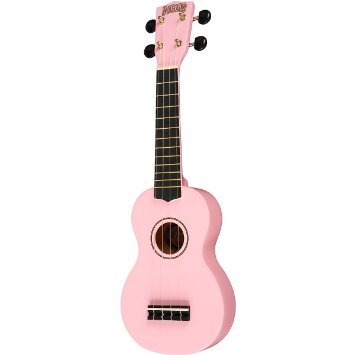
\includegraphics[width=5cm]{../img/ukulele.jpg}
\end{Slide}


% subjekt och predikat -> public static void: https://www.youtube.com/watch?v=1ZPaR_wH-R8


% \begin{Slide}{Koda i Scala}

%   {\footnotesize\it Melodi: McDonalds-låten}
% % https://youtu.be/cTVhZqNwn3Y

% \begin{verbatim}

%           G         C             G          D
% Det finns stunder i livet som man alltid har kvar

%           G           C               D
% Det finns villkor och uttryck som man spar 

%         A           D             A           E
% Och där koden är öppen finns gemenskap för fler 

% A      D      E       A
% Koda i Scala; det ger meeeeeeer! 
% \end{verbatim}

% \end{Slide}



% F        F9   Fmaj7 F9        Fmaj7
% Å detta språk detta ljuvliga språk

% F             Gm    Gm7     C7
% som vi kallar bella Scala

% Gm                 Gm7       C7
% se vilken syn alla uttryck i skyn

%       Gm    C7    F
% detta ljuva bella Scala

% Cm                  Cm7  F7     Bbmaj7        Bb
% fjärran från det du älskar blir koden ödsligt tom

%     Dm7   G7     Dm7      G7        Gm7         C
% men i din närhet sluts du in i dess trolska rikedom

%    F        Am           Eb        D
% åh åh detta språk det är ungdomens språk

%        Gm     C     F      C7       
% som vi kallar bella Scala




\fi
